\documentclass[tikz,border=3pt]{standalone}
\usepackage{amsmath}
\usepackage{xcolor}
\usetikzlibrary{arrows.meta,calc,decorations.pathreplacing,positioning,fit,backgrounds}

\definecolor{cpos}{RGB}{31,119,180}   % class + : blue
\definecolor{cneg}{RGB}{214,39,40}    % class - : red
\definecolor{cmar}{RGB}{44,160,44}    % margin / certificate accent : green
\definecolor{cax}{RGB}{60,60,60}

\begin{document}
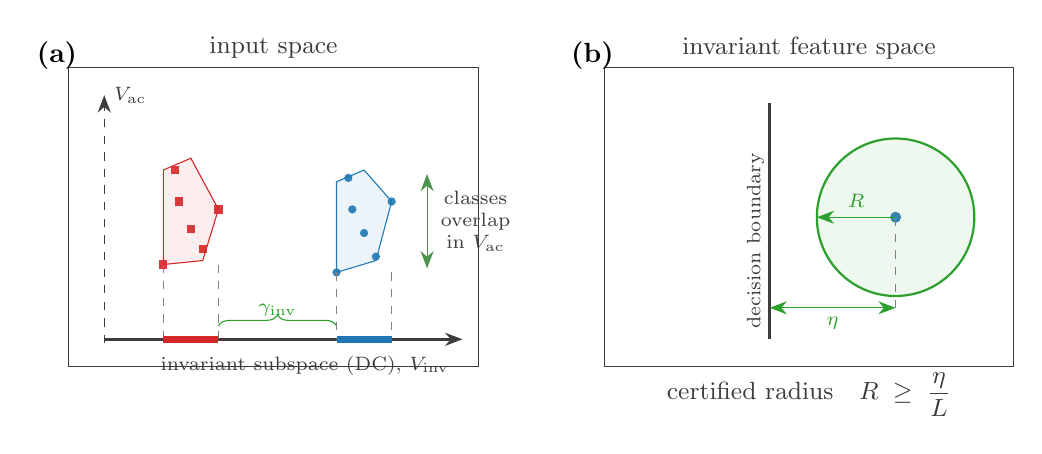
\begin{tikzpicture}[
  >={Stealth[length=2.2mm]},
  poscol/.style={cpos,fill=cpos,fill opacity=0.9},
  negcol/.style={cneg,fill=cneg,fill opacity=0.9},
  drop/.style={gray,very thin,dashed},
]

% ============================ PANEL A: projection geometry ============================
\begin{scope}
  % bounding box (input space)
  \draw[cax,thin] (0,0.6) rectangle (5.2,4.4);
  \node[cax,font=\small] at (2.6,4.65) {input space};

  % AC axis (vertical, dashed, muted) -- invariance is blind to it
  \draw[cax,dashed,->] (0.45,0.9) -- (0.45,4.05) node[right,font=\scriptsize] {$V_{\mathrm{ac}}$};
  % DC / invariant axis (horizontal, bold) -- the projection target
  \draw[cax,line width=1pt,->] (0.45,0.95) -- (5.0,0.95) node[right,font=\scriptsize] {};
  \node[cax,font=\scriptsize] at (3.0,0.62) {invariant subspace (DC), $V_{\mathrm{inv}}$};

  % class - cloud (red squares), left in DC, overlapping in AC
  \foreach \p in {(1.4,2.7),(1.7,2.1),(1.2,1.9),(1.9,2.6),(1.55,2.35),(1.35,3.1)}{
    \node[negcol,rectangle,minimum size=3pt,inner sep=0pt] at \p {};}
  % class + cloud (blue circles), right in DC, overlapping in AC
  \foreach \p in {(3.6,2.6),(3.9,2.0),(3.4,1.8),(4.1,2.7),(3.75,2.3),(3.55,3.0)}{
    \node[poscol,circle,minimum size=3pt,inner sep=0pt] at \p {};}

  % convex hulls (translucent)
  \draw[cneg,fill=cneg,fill opacity=0.08,thin] (1.2,1.9)--(1.2,3.1)--(1.55,3.25)--(1.9,2.6)--(1.7,1.95)--cycle;
  \draw[cpos,fill=cpos,fill opacity=0.08,thin] (3.4,1.8)--(3.4,2.95)--(3.75,3.1)--(4.1,2.7)--(3.9,1.95)--cycle;

  % projection drop-lines onto the DC axis (a few representative points)
  \foreach \x in {1.2,1.9}{ \draw[drop] (\x,1.9) -- (\x,0.95); }
  \foreach \x in {3.4,4.1}{ \draw[drop] (\x,1.8) -- (\x,0.95); }

  % projected intervals on the DC axis
  \draw[cneg,line width=2.5pt] (1.2,0.95) -- (1.9,0.95);
  \draw[cpos,line width=2.5pt] (3.4,0.95) -- (4.1,0.95);

  % gamma_inv gap brace between projected intervals (above the axis, in the empty gap)
  \draw[cmar,decorate,decoration={brace,amplitude=4pt}] (1.9,1.12) -- (3.4,1.12)
     node[midway,above,font=\scriptsize,cmar] {$\gamma_{\mathrm{inv}}$};

  % AC-overlap annotation
  \draw[cmar!60!gray,<->] (4.55,1.85) -- (4.55,3.05);
  \node[cax,font=\scriptsize,align=center,anchor=west] at (4.6,2.45) {classes\\overlap\\in $V_{\mathrm{ac}}$};
\end{scope}

% ============================ PANEL B: eta/L certificate ============================
\begin{scope}[xshift=6.8cm]
  \draw[cax,thin] (0,0.6) rectangle (5.2,4.4);
  \node[cax,font=\small] at (2.6,4.65) {invariant feature space};

  % decision boundary
  \draw[cax,line width=1pt] (2.1,0.95) -- (2.1,3.95);
  \node[cax,font=\scriptsize,rotate=90] at (1.92,2.2) {decision boundary};

  % the data point
  \coordinate (P) at (3.7,2.5);
  \node[poscol,circle,minimum size=4pt,inner sep=0pt] at (P) {};

  % certified ball radius R
  \draw[cmar,fill=cmar,fill opacity=0.08,thick] (P) circle (1.0);
  \draw[cmar,->] (P) -- ++(-1.0,0) node[midway,above,font=\scriptsize,cmar] {$R$};

  % margin eta from point to boundary
  \draw[cmar,<->,thin] (2.1,1.35) -- (3.7,1.35) node[midway,below,font=\scriptsize,cmar] {$\eta$};
  \draw[drop] (P) -- (3.7,1.35);

  % the certificate statement
  \node[cax,font=\small,align=center] at (2.6,0.25)
     {certified radius\quad $R \;\ge\; \dfrac{\eta}{L}$};
\end{scope}

% panel labels
\node[font=\bfseries] at (-0.15,4.55) {(a)};
\node[font=\bfseries] at (6.65,4.55) {(b)};

\end{tikzpicture}
\end{document}
